%File: paper.tex --- AIES 2026 anonymous submission
\documentclass[letterpaper]{article} % DO NOT CHANGE THIS
\usepackage[submission]{aaai2026}    % DO NOT CHANGE THIS
\usepackage{times}    % DO NOT CHANGE THIS
\usepackage{helvet}   % DO NOT CHANGE THIS
\usepackage{courier}  % DO NOT CHANGE THIS
\usepackage[hyphens]{url}  % DO NOT CHANGE THIS
\usepackage{graphicx} % DO NOT CHANGE THIS
\urlstyle{rm}         % DO NOT CHANGE THIS
\def\UrlFont{\rm}     % DO NOT CHANGE THIS
\usepackage{natbib}   % DO NOT CHANGE THIS
\usepackage{caption}  % DO NOT CHANGE THIS
\frenchspacing        % DO NOT CHANGE THIS
\setlength{\pdfpagewidth}{8.5in}  % DO NOT CHANGE THIS
\setlength{\pdfpageheight}{11in}  % DO NOT CHANGE THIS

\usepackage{tikz}
\usetikzlibrary{positioning,arrows.meta,shapes.geometric,fit,backgrounds,calc}
\usepackage{booktabs}

\pdfinfo{
/TemplateVersion (2026.1)
}

\setcounter{secnumdepth}{2}

\title{Engineering-Ethics Scaffolding for Deployed Public-Good AI Mental-Health Systems: A Combined License, Deployment-Pause Posture, and Rule-Coverage CI Pattern}

\author{Anonymous Submission}
\affiliations{}

\begin{document}

\maketitle

\begin{abstract}
\noindent Tens of millions of users now talk to AI systems about their mental health. OpenAI disclosed in October 2025 that roughly 0.15\% of weekly active ChatGPT users (over a million people per week) show explicit suicidal-planning indicators \citep{openai2025strengthening}. The 2025 regulatory environment shifted accordingly: an FTC 6(b) inquiry \citep{ftc2025sixb}, FDA Digital Health Advisory Committee deliberations \citep{fda2025dhac}, an APA Health Advisory \citep{apa2025advisory}, and a Florida federal court ruling in \emph{Garcia v.\ Character Technologies} \citep{garcia2025character} that allowed tort claims against an AI-companion company to proceed past First-Amendment-defense dismissal.

A specific governance gap remains unaddressed. Closed-commercial deployments with internal review (Therabot \citep{heinz2025therabot}, Wysa \citep{inkster2018wysa}, Limbic Access \citep{habicht2024limbic}) keep their governance private. Open-source companion systems generally ship without safety-section retention constraints; the fork-strips-safety failure mode is documented \citep{aiid2023neda}. The literature has no published scaffolding for the third regime: \emph{grassroots public-good} deployments shipped without commercial revenue, without medical-device certification, and without organizational backstop --- yet operating into the same elevated-litigation environment as the regulated systems, and serving the same user population at risk.

This paper proposes, and provides a forkable reference implementation of, the \emph{first published, externally-auditable engineering-ethics scaffolding} designed for that third regime. The package combines three tools, each individually rooted in prior art but, by our search of 25 deployed AI mental-health systems and adjacent research literature, never previously combined for this deployment context: (1)~a section-level restricted-use license on system-prompt text (\texttt{LICENSE-PROMPT.md}) requiring named-section retention and clinical-reviewer-of-record substitution, drawing on Hippocratic-License \citep{hl3}, OpenRAIL \citep{openrail2022}, and MPL \citep{mpl2}; (2)~a public deployment-pause posture with auditable trigger conditions, named adjudicators per trigger, and a calibrated-grace-window operator-unavailability dead-man switch; (3)~a CI-enforced rule-coverage check mapping registered safety rules to behavioral test assertions, drawing on CheckList \citep{ribeiro2020checklist} and bidirectional-traceability practices in safety-critical software. \textbf{System X} is the reference implementation: two of three components are production-active, the third is API-validated pending external-scheduler wiring.

We position the package as a \emph{floor}, not a ceiling: minimum viable scaffolding for grassroots deployments that would otherwise ship with no governance, while higher bars (clinical RCT, FDA SaMD pathway, IRB supervision) are pursued in parallel. The paper does not claim the package substitutes for clinical evaluation, regulatory compliance, or operator liability insurance, that the proposed license has been tested in court, that any external party has yet adopted the pattern, or that the rule-coverage CI catches semantic regressions in the registered rules.
\end{abstract}

\noindent\textit{Throughout this paper we refer to the reference implementation we built as \textbf{System X}, anonymized for double-blind review. Repository, deployment URL, and author identification are withheld; an anonymous code mirror is provided in supplementary materials.}

\section{Introduction}
\label{sec:intro}

\subsection{The Deployment Landscape and the Governance Vacuum}

By late 2025 the deployed AI mental-health landscape had bifurcated into two regimes, neither of which carried an externally inspectable governance package.

The first regime is closed-commercial deployment with internal review. Therabot \citep{heinz2025therabot} was developed under six years of expert-curated CBT corpus construction and ran as an actively-monitored RCT with human safety review of every flagged exchange. Wysa \citep{inkster2018wysa} holds an FDA Breakthrough Device Designation and is integrated into NHS Talking Therapies. Limbic Access \citep{habicht2024limbic} was the first AI mental-health chatbot to gain UKCA Class~IIa medical-device status. These systems have substantive internal governance. The governance is not externally inspectable: the system prompts, the safety SOPs, the trigger conditions, and the review processes are not published. A grassroots developer cannot fork Wysa, and Therabot's weights are not public.

The second regime is open-source release without safety-section retention constraints. Character.AI operates under the open-roleplay paradigm. Replika \citep{maples2024replika} and the open-source mental-health LLMs (MentaLLaMA \citep{yang2024mentallama}, SoulChat, EmoLLM, and adjacent work) ship with varying levels of safety scaffolding but no published constraint that prevents stripping it on fork. The fork-removes-safety failure mode is documented \citep{aiid2023neda}. In mid-2023, the NEDA helpline replaced human counselors with a generative-augmented ``Tessa'' chatbot that produced overt eating-disorder-promoting advice, including 500--1,000 calorie/day deficits recommended to ED-recovery users. After public testing surfaced the harm on May~30 2023, NEDA suspended Tessa within 24 hours, on May~31 2023, before the June~1 scheduled rollout that would have replaced the helpline staff.

The regulatory environment shifted accordingly through 2025. The FTC issued 6(b) orders in September \citep{ftc2025sixb} to Meta, OpenAI, Character Technologies, Alphabet/Google, and others on chatbot companions and youth mental health. The FDA Digital Health Advisory Committee considered generative-AI mental-health devices on November~6, 2025 \citep{fda2025dhac} and recommended Predetermined Change Control Plans, performance monitoring, and double-blind RCTs. The APA issued a Health Advisory the same month \citep{apa2025advisory}. In \emph{Garcia v.\ Character Technologies} \citep{garcia2025character}, Judge Anne Conway's May~20 2025 ruling denied Defendants' motion to dismiss on First-Amendment-defense grounds, allowing negligence, product-liability, wrongful-death, and FDUTPA claims to proceed; only intentional-infliction-of-emotional-distress was dismissed. The case settled on January~7 2026 with terms undisclosed, covering Garcia and a related series of suits in Colorado, New York, and Texas. The settlement is consistent with elevated litigation-risk exposure under Conway's Order, but defendants settle for many reasons that are not equivalent to conceding the substantive question (cost, distraction, discovery exposure), so the Conway ruling rather than the settlement is the substantive precedent on whether chatbot output is shielded from tort liability by the First Amendment. Any deployed AI mental-health system shipping in 2026 operates under expanded operator-liability exposure with no clear regulatory pathway.

What is missing from the published literature is a governance pattern that is inspectable from outside, constraining when forked, and operable by a single developer or small team without commercial revenue. This paper proposes and operationalizes such a pattern.

\subsection{The Gap Specific to Grassroots Public-Good Deployments}

Existing governance approaches presume one of two infrastructures. The first is commercial revenue funding internal review boards, clinical advisory panels, and counsel retention, as in Therabot \citep{heinz2025therabot}, Wysa \citep{inkster2018wysa}, and Limbic Access \citep{habicht2024limbic}. The second is regulatory-pathway compliance under medical-device frameworks (FDA SaMD \citep{fda2017samd}, UKCA Class~IIa) that themselves demand institutional backing. The third regime --- public-good deployments operating without commercial revenue, without medical-device certification, and without organizational backstop --- has no published scaffolding. The literature does not currently distinguish this regime from the open-source-without-retention regime in which forks silently strip safety-critical sections \citep{aiid2023neda}, and consequently offers grassroots builders no governance tooling that survives the fork. This paper articulates the gap and proposes a forkable scaffolding designed to fill it.

\subsection{Three-Tool Package}

The package combines three tools that together compose what we call the \emph{minimum viable} safety scaffolding for this regime. None of the tools is novel individually; each has substantial prior art. The contribution is the documented synthesis: a forkable set of artifacts designed against an articulated governance gap, with a documented prior-art search supporting the claim that no published combination exists for the third regime.

\begin{enumerate}
\item A restricted-use license on system-prompt text (\texttt{LICENSE-PROMPT.md}) that requires named-section retention and reviewer-of-record substitution for derived deployments (\S\ref{sec:license}).
\item A self-imposed deployment-pause posture with auditable trigger conditions, named adjudicators per trigger, and an operator-unavailability dead-man switch (\S\ref{sec:pause}, \S\ref{sec:deadman}).
\item A CI-enforced rule-coverage check mapping registered safety rules to behavioral test assertions (\S\ref{sec:ci}).
\end{enumerate}

Each tool addresses a different governance surface. Figure~\ref{fig:composability} summarizes the resulting composition. The license addresses derivative deployments (forks otherwise silently strip safety-critical sections). The deployment-pause posture addresses the original deployment (the operator's commitment to pause under named conditions is otherwise unenforceable from outside). The rule-coverage CI addresses both, by providing the deterministic safety-rule signal that the pause posture's rule-coverage trigger consumes. The three components do not form a closed enforcement loop. The CI feeds the original deployment's pause posture but does not constrain forks; the license constrains forks but does not gate the original. Closing the loop fully (for instance, by requiring under the proposed license that forks ship with an equivalent CI configured against their derived spec) is one direction of future-work refinement we flag in \S\ref{sec:discussion} and do not claim as part of this paper's package.

\begin{figure*}[t]
\centering
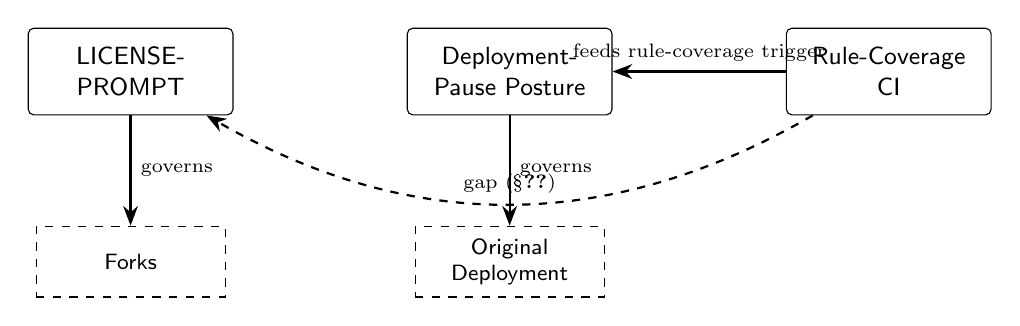
\begin{tikzpicture}[
  >={Stealth[length=2.5mm]},
  node distance=8mm,
  box/.style={rectangle, draw, rounded corners=2pt, minimum width=26mm, minimum height=11mm, align=center, font=\small\sffamily, inner sep=2pt},
  smallbox/.style={rectangle, draw, dashed, minimum width=24mm, minimum height=9mm, align=center, font=\footnotesize\sffamily, inner sep=2pt},
  arrow/.style={->, thick},
  weakarrow/.style={->, thick, dashed},
  font=\small,
]
  % Tools row
  \node[box] (license) {LICENSE-\\PROMPT};
  \node[box, right=22mm of license] (pause) {Deployment-\\Pause Posture};
  \node[box, right=22mm of pause] (ci) {Rule-Coverage\\CI};

  % Targets
  \node[smallbox, below=14mm of license] (forks) {Forks};
  \node[smallbox, below=14mm of pause] (orig) {Original\\Deployment};

  % Arrows: tool -> surface
  \draw[arrow] (license) -- (forks) node[midway, right, font=\scriptsize] {governs};
  \draw[arrow] (pause) -- (orig) node[midway, right, font=\scriptsize] {governs};

  % CI -> pause (the closing direction we have)
  \draw[arrow] (ci) -- (pause) node[midway, above, font=\scriptsize, align=center] {feeds rule-coverage trigger};

  % CI -> license (the gap)
  \draw[weakarrow] (ci) to[bend left=30] node[above, font=\scriptsize] {gap (\S\ref{sec:discussion})} (license);
\end{tikzpicture}
\caption{The three-tool package composes against complementary governance surfaces but does not form a closed enforcement loop. Solid arrows: enforced relations. Dashed arrow: the acknowledged gap between rule-coverage CI and the license's fork-constraint clause.}
\label{fig:composability}
\end{figure*}

\subsection{What This Paper Is and Is Not}

This paper is a governance-pattern proposal with one reference implementation and a documented prior-art search. The reference implementation is System~X: two of three components are production-active, the third is API-validated pending external-scheduler wiring. The paper is not a clinical-evaluation paper (System~X has no published RCT and is not FDA-cleared), not a regulatory-compliance pathway (the deployment is positioned outside regulated medical-device categories, which \S\ref{sec:limitations} lists as a limitation), and not legal advice (the proposed license has not been tested in court). Empirical work on the substrate-level anti-pattern catalog and a measurement-validity reading of the VERA-MH benchmark \citep{bentley2026veramh} is deferred to separate work in preparation.

\section{The Three-Tool Package}
\label{sec:package}

\subsection{LICENSE-PROMPT: Use-Restricted System Prompt Sections}
\label{sec:license}

A deployed AI mental-health system's safety behavior is encoded primarily in its system prompt: crisis-trigger logic, forbidden utterances, imminent-risk handling, referral resources. MIT-style permissive release lets forks both improve the prompt and strip safety-critical sections. A README note asking forks not to strip is unenforceable; a copyright-license-level constraint is.

\texttt{LICENSE-PROMPT.md} governs \texttt{src/lib/system-prompt.ts} and substantially-derivative prompts. It grants broad redistribution, modification, and commercial-use rights with carve-outs for four named sections. \S1.a is the imminent-risk SOP (method-driven persuasion plus means restriction plus companion-during-call). \S1.b is the leverage-prevention rule (no weaponization of named reasons-for-living). \S1.c is the no-third-party-characterization rule (no escalating user's framing of partner, parent, or friend). \S1.d is the companion-during-call requirement, designated \emph{preserved-pending-clinical-validation}. A derived deployment modifying any of these sections must publicly name a clinical reviewer-of-record (defined as holding active state licensure in a clinical mental-health discipline with crisis-intervention experience), document the modification, and publish the modified text. Derived deployments that retain these sections inherit the deploy-pause posture described in \S\ref{sec:pause}.

The fourth section requires a different framing than the others. Companion-during-call is grounded in crisis-line warm-handoff literature \citep{gould2007hotline,mishara2008samaritans} but has not been validated for AI-companion-during-call interactions specifically. Locking an under-evidenced protocol via copyright would be paradoxical if read as ``established practice.'' We read it instead as a protection against silent stripping, with license substitution available under a transparency requirement: the reviewer-of-record path in \texttt{LICENSE-PROMPT} \S2 is the explicit update channel for substantive modifications. A fork engaging a clinical reviewer-of-record may modify \S1.d freely under \S2 terms. What the license blocks is silent removal by forks that have done no clinical evaluation. The same asymmetric standard applies to the original System~X deployment. The clinician-review trigger commits System~X itself to obtaining the same review on a public 2026-06-30 deadline, with deployment-pause consequences if missed. Status (and any post-deadline update) is committed to a public auditable artifact in the project repository.

LICENSE-PROMPT combines three prior patterns. From the Hippocratic License v3 \citep{hl3}, it inherits the use-restriction approach; HL3 has over 300 adopters, none of them deployed AI mental-health systems. From the OpenRAIL-M family \citep{openrail2022}, it inherits the behavioral-constraint approach, although OpenRAIL applies to model weights and LICENSE-PROMPT applies to prompt text. From Mozilla MPL v2 \citep{mpl2}, it inherits file-level copyleft, although MPL targets the file as a whole and LICENSE-PROMPT targets named sections within a file. The combination of section-level retention, a reviewer-of-record substitution clause, and application to a deployed AI mental-health system's prompt is, by our search in \S\ref{sec:priorart}, not previously published.

LICENSE-PROMPT has substantial limitations, listed in \S\ref{sec:limitations}. Enforceability has not been tested in court, the legal quality has not been reviewed by counsel, and the reviewer-of-record substitution mechanism creates a gating step that some adopters may treat as friction rather than feature. A lawyer's review is the most important external obligation on the tool.

\subsection{Deployment-Pause Posture with Auditable Triggers}
\label{sec:pause}

The phrase ``we will pause the deployment if something goes wrong'' is unenforceable as a public commitment because both ``something goes wrong'' and ``we will pause'' are operator-discretionary. A monitoring-without-trigger commitment cannot be audited from outside, and neither can a trigger that lacks named adjudicators or deadlines. The pause posture has to be specific enough that an external reviewer can check whether the operator actually paused when they said they would.

System~X commits to four trigger conditions, summarized in Table~\ref{tab:triggers}. Each has a named adjudicator, a defined adjudication artifact, and a time bound.

\begin{table}[t]
\small
\centering
\caption{Deployment-pause triggers for System~X.}
\label{tab:triggers}
\begin{tabular}{@{}p{1.5cm}p{2.0cm}p{1.4cm}p{1.5cm}@{}}
\toprule
Trigger & Adjudicator & Window & On Fire \\
\midrule
Clinician review & Operator $\rightarrow$ ext.\ clinician for resume & Deadline 2026-06-30 & Feature flag off; ``research preview'' \\
Sentinel adverse event & Operator (verify) $\rightarrow$ clinician (resume) & 24h after verification & Referral-only \\
Rule-coverage gap & CI (deterministic) & 30 days & Pause until restored \\
Legal demand & Operator $\rightarrow$ counsel (resume) & 72h verify, then 24h & Referral-only \\
\bottomrule
\end{tabular}
\end{table}

The \emph{clinician-review trigger} fires if no licensed clinician has provided written review of at least one of the imminent-risk SOP, the companion-during-call protocol, the leverage-prevention rule, or the per-population SOPs by 2026-06-30. On firing, the companion-during-call feature and the method-driven imminent-persuasion SOP move behind a default-off feature flag, and the deployment's positioning text changes from product-mode to ``research preview, not for use during active distress.'' The adjudicator is the operator. The clinician sign-off, or its absence, is committed to a public clinician-audit artifact by 2026-07-07.

The \emph{sentinel adverse event trigger} fires on a verified credible report of suspected user death, near-death, or severe iatrogenic harm. Verification requires both a reporting party with confirmable identity (licensed clinician, documented family member, law enforcement, or masthead media organization) and independent confirmation of the specific circumstance. The deployment enters referral-only mode within 24 hours of verification, pending external review. The pause is invoked manually by setting the heartbeat-store gate to \texttt{expired} (the same substrate the dead-man switch uses; see \S\ref{sec:deadman}); it is not an automated pipeline. The adjudicator is the operator for the manual pause, and an external clinician reviewer for the resume decision. Receipt-side automation, a soft-pause-banner on plausibly-credible reports prior to verification with rate-limiting and de-duplication against griefer-spam, is a v0.9 milestone. Single-operator adjudication is the residual exposure; multi-party HMAC threshold signing once a clinician-of-record is engaged is the natural v1 hardening.

The \emph{rule-coverage trigger} fires if \texttt{npm run check-rule-coverage} shows critical-rule coverage gaps unresolved for more than 30 days. The deployment is paused until coverage is restored. The adjudicator is the CI check itself, which is deterministic. Enforcement is live as merge-blocking branch protection. A runtime kill-switch (a \texttt{DEPLOY\_GATE\_OPEN} env var consumed in the chat route, which would immediately move the deployed instance to referral-only mode on CI failure rather than only blocking new merges) is a v0.9 milestone.

The \emph{legal-demand trigger} fires on a verified credible legal demand related to user safety: a subpoena or regulatory inquiry from the FTC, FDA, or a state AG (verified via PACER, the regulator's docket, or direct phone confirmation to the issuing office); a tort complaint filed in court (PACER-checkable); or a cease-and-desist from counsel-of-record (firm verified in the state bar registry). On verification, the deployment enters referral-only mode within 24 hours, pending counsel review. The verification window is 72 hours from receipt. Same-day verification by a single uninsured operator would frequently produce false-positive pauses on malformed or fraudulent demands. Unverified-pending-72h demands get a soft-pause warning banner without the hard pause. The adjudicator is the operator for the post-verification pause and counsel for the resume decision.

Each trigger is committed in a public deployment-conditions registry along with the named adjudicators, deadlines, and any past invocations. A skeptical reviewer can verify operator compliance on any date. The closest published precedents are research-trial deployment protocols, including Therabot's IRB-supervised pause-on-flag practice \citep{heinz2025therabot} and Wysa's clinical advisory board \citep{inkster2018wysa}, and the safety-cases tradition in safety-critical software engineering \citep{rtca2011do178c, sae1996arp4761}, in which named conditions and adjudicators are required for certification but not for ordinary operation. We adapt the named-conditions-and-adjudicators pattern from safety-cases to ordinary operator-self-restraint, without the certification scaffolding. To our knowledge, no published deployed AI mental-health system commits to a public, auditable, trigger-and-adjudicator deployment-pause posture of this form.

\subsection{Operator-Unavailability Dead-Man Switch}
\label{sec:deadman}

The deployment-pause posture in \S\ref{sec:pause} names the operator as the adjudicator on two of the four triggers. This creates a single point of failure. If the operator is unavailable through illness, travel, or abandonment, the deployment continues operating without the adjudication mechanism that justifies its operation.

Our first-pass design used a scheduled GitHub Actions workflow checking last-commit-age. GitHub auto-disables scheduled workflows in public repositories after 60 days of inactivity, which defeats the trigger precisely when sustained inactivity is the firing condition. We flag this pitfall explicitly so other AI mental-health projects do not repeat it.

The replacement design uses signal-loss-default-deny with a calibrated grace window. An external cron-as-a-service provider, independent of the project repo and the deployment platform, fires a daily HMAC-SHA256-signed heartbeat to \texttt{/api/admin/heartbeat}. The endpoint validates a $\pm$10-minute drift window for replay protection and uses \texttt{timingSafeEqual} for signature comparison. On each request, the deployment computes \texttt{now -- last\_heartbeat} and returns one of three statuses: \texttt{healthy} ($\le$48~hours), \texttt{warning} (48~hours to 7~days, with a banner added to the response), or \texttt{expired} (more than 7~days, request returns referral-only). The 7-day cutoff is calibrated to single-operator normal life. Weekend illness, family emergency, and international travel routinely produce 48--72-hour gaps, and a tighter cutoff would fail-closed a safety-critical service on the typical case. Beyond 7~days, the deployment fails closed regardless of why the heartbeat stopped.

The mechanism has substantial limits on the infrastructure side. Persistence: \texttt{last\_heartbeat\_at} is module-level state, so serverless cold-starts reset to ``unknown'' (which the chat-route consumer treats as healthy by design). Production-grade persistence is a v0.9 milestone. Independence is only partial: the operator configures the cron, holds the HMAC secret, and can disable the cron from the same machine that writes the system prompt. The redesign relocates the single point of failure from GitHub-Actions infrastructure to cron-provider infrastructure rather than removing it. The mechanism defends against unavailability, not against adversarial action. Multi-party HMAC threshold signing across the operator, a clinician reviewer, and a neutral third party is the natural v1 hardening once a clinician-of-record is engaged.

The clinical-side limit is sharper. Fail-closed-during-crisis versus degraded-availability is a live clinical question: a user in \texttt{expired} mode at 3~AM receives a referral-only response naming 988, Crisis Text Line, and 911 instead of System~X's companion protocol. The 7-day grace plus 48-hour warning configuration was chosen over a tighter 48-hour pause precisely to minimize this exposure on the typical case. The right calibration on the boundary case is unsettled pending clinical reviewer-of-record input.

Deployed-system dead-man switches in AI mental health, defaulting to referral-only on operator-unavailability, are not standard practice and we have not located prior published examples. The contribution here is the framing of ``fail closed on signal loss'' as the correct default for safety-critical deployed AI, the GitHub-Actions self-disabling finding as transferable engineering knowledge, and the integration with \S\ref{sec:pause}'s trigger structure.

\subsection{Rule-Coverage CI}
\label{sec:ci}

\noindent\textbf{The problem.} Behavioral testing of LLM systems with templated assertions \citep{ribeiro2020checklist} catches regressions on assertions that were written, but does not catch the case where a safety rule was added to the system prompt but no test was written for it. The rule-test mismatch is the main maintenance hazard in deployed safety-critical conversational systems: a rule that nominally exists in the prompt but has no test will silently regress on prompt-update or model-update.

A hand-maintained \texttt{REQUIRED\_RULES} registry enumerates the safety rules that must have at least one critical-severity behavioral assertion testing them. Each scenario in the test suite (61 scenarios at the time of writing) contains assertions; each critical-severity assertion carries a \texttt{rule:} field naming which \texttt{REQUIRED\_RULES} entry it tests. The \texttt{npm run check-rule-coverage} script enforces, for every entry in \texttt{REQUIRED\_RULES}, that at least one critical assertion references it. The check runs in CI and fails the build if coverage drops to zero on any rule. Adding a new rule to \texttt{REQUIRED\_RULES} without writing an assertion fails CI immediately, as does removing all assertions for a rule or renaming an assertion's \texttt{rule:} field without updating the registry.

What the check does not catch is the converse: adding a new rule to the system prompt without registering it in \texttt{REQUIRED\_RULES} is silent. The registry is hand-maintained, and there is no automated check that rules-in-prompt is a subset of rules-in-registry. Beyond this omission gap, the current spec contains five items deliberately not registered: three named safety rules (\texttt{inviolable.3} ``never assert another's intent,'' \texttt{inviolable.7} ``no comparison to others, even favorably,'' and \texttt{protocol.8} ``rupture/repair check-in''), and two agency-trajectory functions (\texttt{agency.memory} ``long memory plus pattern surface'' and \texttt{agency.logger} ``structured journaling''). These five require test infrastructure not yet built: long-conversation scenarios for \texttt{protocol.8} and the rupture-check, and a multi-session harness for the two agency-affordance functions. They are documented as TODO with prefix-comments in the registry source. The CI check on the registered rules passes; the registry-omission gap is openly disclosed both in the source comments and in the public deployment-conditions artifact. Semantic adequacy is also not checked: an assertion can pass while the rule it nominally tests is misimplemented in the prompt.

The methodology root is CheckList's MFT/INV/DIR three-test-type taxonomy \citep{ribeiro2020checklist}. The conceptual root for rule-to-test mapping is bidirectional traceability in safety-critical software \citep{rtca2011do178c, iso2018iso26262, fda2023premarket}. We borrow loosely from both: templated behavioral assertions from CheckList, and registry-driven coverage checking from safety-critical traceability. This is a v1 partial implementation; it does not approach the verification depth those standards demand. CheckList has been applied to many domains, but we have not located a published application to clinical safety rules in deployed AI mental-health systems with registry-driven coverage gating in CI. Adjacent work in this space (MentaLLaMA \citep{yang2024mentallama}, role-aware safety evaluations \citep{lee2026mhsafeeval}) tests classifier accuracy or QA quality; rule-coverage as a deployment-gating CI check is, to our knowledge, new in this domain.

\section{System X as a Reference Implementation}
\label{sec:systemx}

\subsection{Architecture Summary}

System~X is a Next.js~15 web application backed by a vendor LLM. The system prompt (\texttt{src/lib/system-prompt.ts}, $\sim$6,500 tokens at the current version) is injected on every conversation. User conversations are stored in IndexedDB, encrypted with AES-GCM-256 using a key the browser holds; the server cannot read conversation content. Default retention is 90 days, user-configurable. Crisis tooling, panic-phrase quick-exit, and Stanley-Brown stabilization-window safety planning \citep{brown2018spi} are implemented in client-side React components.

\subsection{LICENSE-PROMPT in Practice}

The system prompt file (\texttt{src/lib/system-prompt.ts}) opens with a TypeScript-comment license header referencing \texttt{LICENSE-PROMPT.md}. The four named protected sections inside the prompt's template-literal body are explicitly delimited by HTML-style comments visible in the raw text (\texttt{<!-- PROTECTED SECTION: imminent-risk SOP -- see LICENSE-PROMPT.md \S1.a -->} through the matching close marker). The HTML-comment form is used because it survives unchanged through markdown rendering by clients while remaining greppable from the file system; TypeScript-comment markers (\texttt{//}) would not work inside the template literal. A derived fork that removes these comment markers removes the in-text indication of which sections are protected but the license still applies; the canonical mapping of sections to license clauses lives in \texttt{LICENSE-PROMPT.md}, not in the prompt comments.

The reviewer-of-record substitution clause has not been invoked at the time of writing --- no fork has been documented to the project. The clause's first test will be when one occurs.

\subsection{Deploy-Pause Triggers Wired Up}

The rule-coverage trigger is currently enforced via repository branch protection: a workflow runs \texttt{npm run check-rule-coverage} on every push and pull request to main, and a coverage-gap failure blocks merge. A \emph{runtime} kill-switch --- a \texttt{DEPLOY\_GATE\_OPEN} env var consumed in \texttt{src/app/api/chat/route.ts} that would pause the running deployment immediately on CI failure (rather than only blocking new merges) --- is a v0.9 milestone and is not yet wired. The dead-man-switch heartbeat gate (\S\ref{sec:deadman}) \emph{is} live as a runtime gate; the rule-coverage gate is currently merge-time only.

The dead-man switch is implemented as the signal-loss-default-deny-with-grace-window pattern described in \S\ref{sec:deadman}. The deployment-side consumer at \texttt{src/app/api/admin/heartbeat/route.ts} accepts POSTs of \texttt{\{timestamp,~signature\}} JSON bodies, verifies HMAC-SHA256 against a secret env var with a $\pm$10-minute drift window for replay protection and \texttt{timingSafeEqual} for signature comparison, and writes the timestamp to the heartbeat store at \texttt{src/lib/heartbeat-store.ts}. The store exports \texttt{getHeartbeatStatus()} which returns \texttt{healthy} / \texttt{warning} / \texttt{expired} / \texttt{unknown} per the 7-day validity / 48-hour warning windows. The chat route at \texttt{src/app/api/chat/route.ts} calls \texttt{getHeartbeatStatus()} immediately after the daily-cap check and (a)~returns a referral-only 503 response when status is \texttt{expired}, and (b)~emits a \texttt{heartbeat\_status} SSE event with a warning-banner payload when status is \texttt{warning} so the client renders the operator-may-be-unavailable notice above the conversation. The external scheduler component (a third-party cron service firing the daily heartbeat against the deployment URL) is the cron-side wiring task and is not part of the project repository.

\noindent\textbf{Current operational status:} the deployment-side endpoint, store, gate, and warning-banner SSE emission are implemented and validated. The external scheduler is \emph{not yet configured} at the time of this paper's writing --- the mechanism is therefore in \emph{demo / API-validated} state, not in \emph{production-active} state. Until the cron is configured, the deployment runs in \texttt{unknown} heartbeat status (treated as healthy per the cold-start semantic in \texttt{src/lib/heartbeat-store.ts}). We surface this gap explicitly because a hostile reviewer would otherwise catch it by clicking through to the public deployment-conditions artifact.

The clinician-review and sentinel-event triggers are operator-discretionary at the moment of trigger and committed-to-repo as auditable artifacts after.

\subsection{The 61-Scenario Test Suite Plus Rule-Coverage Check}

The test suite (\texttt{scripts/scenarios/}) contains 61 scenarios across 13 categories (suicide, DV, leverage, trauma, psychosis-mania, OCD, ED, substance, threats, caregiver, daily, calibration, parasocial). Each scenario contains a sequence of user turns and a list of behavioral assertions. Six assertion kinds are supported: \texttt{must\_call\_tool}, \texttt{must\_not\_call\_tool}, \texttt{must\_match} (regex pattern present), \texttt{must\_not\_match} (pattern absent), \texttt{max\_occurrences} (pattern bounded), \texttt{judge} (LLM-as-judge evaluates yes/no proposition).

\texttt{scripts/check-rule-coverage.ts} enforces the rule-to-assertion coverage. The current \texttt{REQUIRED\_RULES} registry contains 33 rules; the script reports \texttt{33 covered, 0 uncovered} at the time of writing. Five spec rules are \emph{deliberately not registered} (\texttt{inviolable.3}, \texttt{inviolable.7}, \texttt{protocol.8}, \texttt{agency.memory}, \texttt{agency.logger}) pending test infrastructure; their TODO status is documented in the registry source comments.

The full suite (judges enabled, 3-concurrency) runs in 12--18 minutes wall-clock at \$3--6 per pass on the underlying model. \texttt{--no-judge} mode for programmatic-only assertions runs at \$0.50 per pass and is the mode CI uses.

\section{Prior Art and Search Methodology}
\label{sec:priorart}

\subsection{Documented Search}

The novelty claim depends on a defensible search. We searched (2026-04-15 to 2026-04-29): arXiv (cs.HC / cs.CY / cs.AI / cs.CL / cs.SE), ACM DL, IEEE Xplore, JMIR archives, PubMed, the Hippocratic License registry, the OpenRAIL registry, and GitHub topic searches (\texttt{mental-health}, \texttt{chatbot}, \texttt{safety}, \texttt{license}, \texttt{deployment-pause}). Search-term combinations: ``AI/LLM/chatbot mental health'' $\times$ ``system prompt license / prompt restricted use / Hippocratic License / OpenRAIL / CheckList / deployment pause / dead-man switch / rule coverage / safety.''

\noindent\textbf{What we found.} About 25 deployed AI mental-health systems were reviewed (Therabot, Wysa, Limbic Access, Replika, Character.AI, Woebot, Pi, Earkick, Mindstrong, Tessa-NEDA, MentaLLaMA, SoulChat, EmoLLM, ChatPsychiatrist, Mental-LLM, X2AI Tess, Youper, Yana, Pixel.bot, Talkspace AI, BetterHelp AI, Lasting AI, Sintelly, Sonia, Wysa NHS); about seven have peer-reviewed evaluation. Of all 25, \emph{zero} publish their full system prompt, \emph{zero} publish trigger-condition + adjudicator commitments, and \emph{zero} publish a rule-coverage CI artifact tied to a registered rule set. HL3 adopters span analytics / infrastructure / developer-tools but none deployed AI mental-health; OpenRAIL is applied to model weights, not prompts; about five papers apply CheckList-family methodology to LLM mental-health evaluation (MentaLLaMA evaluation, PsyEval, MHSafeEval \citep{lee2026mhsafeeval}, FAITA-MH \citep{golden2024faitamh}, VERA-MH \citep{bentley2026veramh}), none with a CI-gated rule-coverage registry. Research-trial protocols (Therabot IRB pause-on-flag) and regulated medical-device safety cases (DO-178C, ARP4761) embody auditable-trigger patterns privately, not as public commitments for ordinary operation.

\noindent\textbf{Combination claim.} Across all corpora, zero published deployed AI mental-health systems combine all three tools. The novelty claim is made against an empty intersection.

\noindent\textbf{What we cannot rule out.} Internal governance documents at closed-commercial deployments are not public; trade-press venues are not exhaustively searched. We treat the claim as ``no published deployed-system equivalent,'' not ``no equivalent exists anywhere,'' and invite correction.

\subsection{What We Explicitly Do Not Claim Is Novel}

HL3-style use-restriction (since 2020); OpenRAIL behavioral constraint on ML weights (since 2022); MPL file-level copyleft (decades); CheckList behavioral-testing methodology \citep{ribeiro2020checklist}; bidirectional traceability in safety-critical software; auditable trigger conditions in regulated medical-device development; open-source AI mental-health systems (MentaLLaMA, SoulChat, ChatPsychiatrist). What is novel is the \emph{combination} applied to a free, public-good, single-operator AI mental-health deployment, with the proposed license targeting safety-critical sections within a system prompt over a vendor base model.

\subsection{Adjacent Work That Could Be Confused with Our Claim}

\noindent\textbf{Wysa's UKCA Class~IIa medical-device status} \citep{habicht2024limbic} is a regulatory pathway, not a governance package; closed-source, does not publish prompt / triggers / coverage check. \textbf{Therabot's IRB-supervised trial} \citep{heinz2025therabot} had internal governance but is not publicly documented in transferable-pattern form; weights and prompt are not public. \textbf{Anthropic's well-being interventions} \citep{anthropic2025wellbeing} --- sycophancy reduction, self-harm classifier, ThroughLine resource partnership --- operate at the model-vendor / substrate level. System~X's three-tool package operates at the application-deployment level above the substrate; the two layers are complementary.

\noindent\textbf{The Stade et al.\ READI framework} \citep{stade2024readi} for responsible LLM deployment in behavioral healthcare is a vocabulary and stage model, not a tool package. READI provides language for \emph{what} deployment readiness looks like across its proposed stages; our package proposes \emph{how} a public-good deployment can address some of those readiness criteria with concrete artifacts. We position the work as offering tooling that addresses parts of READI's governance vocabulary (specifically: the ``responsible deployment,'' ``ongoing monitoring,'' and ``harm response'' dimensions) without claiming our work constitutes READI-stage compliance --- the framework is more comprehensive than the slice our three-tool package addresses.

\section{Limitations}
\label{sec:limitations}

The pattern's portability is asserted, not demonstrated. As of submission, no external party has adopted the three-tool package or any of its components for an AI mental-health deployment of their own. The proposed license has not been tested in court and the legal text has not been reviewed by counsel. The file-level copyleft mechanism may interact poorly with derivative-work doctrine, and the reviewer-of-record-substitution clause may be challenged as unduly burdensome. Pro-bono review from open-source-license counsel (Software Freedom Conservancy, EFF, university clinics) is being actively sought.

The operator is unincorporated and uninsured. There is no LLC, no errors-and-omissions or cyber-liability coverage, and no prior legal-demand experience. The deploy-pause legal-demand trigger described in \S\ref{sec:pause} is responsible operator behavior, but it does not substitute for incorporation and counsel retention. Readers considering this pattern as a fork base should not infer that operating without these protections is recommended.

The rule-coverage CI is a v1 partial implementation. All 33 rules in the registry are covered, but five spec items are deliberately omitted from the registry pending test infrastructure (\S\ref{sec:ci}). The check is one-directional and does not verify semantic adequacy. Adverse-event monitoring is structurally limited by the local-only encrypted memory architecture. Defensible substitutes (anonymized rule-compliance telemetry, opt-in outcome surveys, sentinel-event reporting, IRB-supervised research partnership) are substitutes, not equivalents. This is the central unsolved problem of the deployment.

System~X deploys to US users in English. The adjudicator names, the legal-demand-trigger agencies, and the proposed license's copyright-law references are all US-specific. International forks would need to remap each.

\section{Discussion and Invitation}
\label{sec:discussion}

\subsection{What We Are Claiming}

The three-tool package is offered as one reference implementation of one possible governance pattern for deployed public-good AI mental-health systems. We claim its components have substantial prior art, and that the combination applied to this deployment context is, by our search, not previously published. We do not claim it is the only possible pattern, that it is optimal, that the reference implementation is fully production-active (the heartbeat external scheduler wiring is the open v0.9 task), or that adopting it suffices for clinical-grade safety. The pattern is the contribution; System~X is an instance.

\subsection{What We Want Others to Do}

We invite others to fork or improve LICENSE-PROMPT. The drafting was done without legal counsel and the reviewer-of-record-substitution clause was designed without enforcement testing. A second draft from someone with open-source license expertise would strengthen the pattern significantly. We will not treat such a fork as competition; the closer the field gets to a standard use-restricted prompt license for safety-critical sections, the better for everyone deploying.

We invite improvements to the deploy-pause trigger taxonomy. Our four triggers reflect the threats we currently see and are not exhaustive. Specific gaps that might warrant additional triggers include data-breach disclosure obligation, model-vendor change of terms (a vendor policy update affecting System~X's substrate, for example), and funding-runway exhaustion. The last is a real condition for any public-good deployment without commercial revenue; Woebot's June 2025 D2C shutdown is the recent precedent. Builders deploying under different threat models will need different triggers.

We invite adoption and improvement of the rule-coverage CI. The check is small, about 150 lines of TypeScript. Bidirectional checking (verifying that all rules-in-prompt have entries in \texttt{REQUIRED\_RULES}) is a natural v2 extension that would close the silent-addition gap \S\ref{sec:ci} acknowledged. Semantic-adequacy verification (whether the assertion actually tests what the rule means) is a much harder open problem and likely requires LLM-as-judge over rule-text and assertion-text pairs.

\noindent\textbf{A note on the open loop between CI and license.} \S\ref{sec:intro} acknowledged that the rule-coverage CI does not currently constrain forks, and that we offer the three tools as composable but not closed-loop. A previous draft of this paper proposed amending LICENSE-PROMPT to require forks to ship an equivalent rule-coverage CI configured against their derived spec. We walked that proposal back. LICENSE-PROMPT's enforceability ceiling is already low (see \S\ref{sec:limitations}), and adding a ``must ship CI we approve of'' clause would do three things, all bad: it would make the license materially more burdensome to comply with, it would require the licensor to evaluate whether each fork's CI is ``equivalent'' (a subjective standard that invites disputes), and it would increase the surface area for the license to be challenged as unduly restrictive. The right direction is to keep LICENSE-PROMPT minimal and defensible (named-section retention plus reviewer-of-record substitution, full stop) and to publish the rule-coverage CI script independently so adopters can choose to run it. Forks that want equivalence can adopt the script; forks that don't are still constrained by LICENSE-PROMPT's section-retention clause. The arrow we hoped to close (CI $\rightarrow$ license $\rightarrow$ fork) is genuinely missing, and we now treat it as a structural property of the package rather than a hole to plug.

\noindent\textbf{Document forks.} A small registry of deployments operating under the package would be valuable as an external accountability artifact. We will host such a registry in the project repository, accept pull requests, and treat inclusion as a governance handshake (the fork enters the same auditable-pause posture as the original).

\subsection{The Scope Honestly Stated}

This paper does not solve deployed AI mental-health safety. It does not approach the regulatory-evidence bar that the FDA SaMD pathway demands \citep{fda2017samd}, the clinical-evidence bar that JMIR Mental Health peer review demands, or the operational-monitoring bar that sentinel-event reporting demands. It offers one engineering-ethics scaffolding pattern that a public-good deployment can adopt as the \emph{minimum viable} governance package while pursuing those higher bars in parallel. We are explicit that \emph{minimum viable} is not \emph{sufficient}: a fork that adopts this package and stops there is not, in our view, operating responsibly. The package is a floor, not a ceiling. The deployment we built (System~X) is operating against this floor in part because the alternative --- operating without any of these scaffolds --- is what most public-good or grassroots AI mental-health deployments currently do. We propose a floor the field can hold each other to.

\section*{Ethical Statement}

This paper proposes a governance package for AI mental-health systems whose users are, by deployment context, often at elevated psychological risk. Three axes warrant explicit ethical discussion.

\noindent\textbf{On the operator-self-restraint framing.} The paper's central proposal --- that a single operator can credibly bind themselves to public auditable trigger conditions --- is, by construction, weaker than third-party regulation. We advocate for the package as a \emph{floor} for grassroots deployments that would otherwise ship with no governance, not as a substitute for regulated medical-device pathways or clinical evaluation. The risk we are trying to mitigate is that ``minimum viable governance'' is read by adopters as ``sufficient,'' which \S\ref{sec:discussion} explicitly disclaims. We have written the limitation into both the paper and the public deployment-conditions artifact.

\noindent\textbf{On the prompt-license enforceability claim.} LICENSE-PROMPT as currently drafted has not been reviewed by counsel and has not been tested in court. The failure mode if a fork strips a protected section and the license is later found unenforceable is that the protected section is, in fact, removed and the user-facing safety behavior degrades. We disclose this in \S\ref{sec:limitations} and treat counsel review as an outstanding obligation rather than an optional refinement. Publishing the pattern before that review carries a risk of legitimating an untested mechanism; we judged the alternative (privately holding a partially-validated pattern that other deployments could benefit from) to be worse, and surface this judgment for reviewer consideration.

\noindent\textbf{On the use of a deployed system in research.} System~X is operated as a public deployment, not a research instrument. Conversation contents are local-only and end-to-end encrypted client-side; the operator cannot read user conversations. The reference-implementation claims in \S\ref{sec:systemx} are therefore based on what the deployment is \emph{configured to do} (verifiable from source) rather than measured \emph{user outcomes}. This limits empirical claims and is acknowledged as the central unsolved problem in \S\ref{sec:limitations}.

\noindent\textbf{Dual-use considerations.} The deployment-pause posture and dead-man switch patterns are general engineering techniques and could be applied to AI deployments outside mental health. We do not see plausible adversarial applications of the rule-coverage CI specifically. The proposed license's reviewer-of-record substitution clause could in principle be adopted by closed-commercial deployments to limit derivative competition; we view this as unlikely in practice (closed deployments do not publish prompts) but flag it as a possible misuse path. The argument of the paper does not depend on the operator being uniquely well-positioned to make these claims; the package is offered for fork or rejection.

\section*{Positionality}

The author of this paper is a single independent developer with no clinical training, no institutional affiliation, no formal background in mental-health research, and no prior peer-reviewed publication in AI ethics or governance. The work is unfunded, operating without institutional review, without IRB supervision, and without clinical advisors at the time of submission. Active outreach to clinical reviewer-of-record candidates and academic research partners is in progress; no engagement is yet finalized.

This positionality shapes the paper in three concrete ways.

\noindent\textbf{The framing of ``minimum viable governance''} as a floor for grassroots deployments is itself shaped by the author's experience as a grassroots deployer rather than as a regulated-medical-device team. A clinically-trained or institutionally-affiliated author would likely have proposed a more conservative posture (e.g., refusing to deploy without IRB) rather than a less conservative one (deploying with self-imposed scaffolding). We disclose this so that readers can read the proposal as one positioned attempt at the trade-off rather than as a neutral analysis. The \S\ref{sec:discussion} acknowledgement that ``minimum viable is not sufficient'' is meant to carry the weight of this positional bias explicitly.

\noindent\textbf{The choice of which prior art to cite} reflects what the author was able to find and read carefully in the search window described in \S\ref{sec:priorart}. Adjacent work in clinical psychology, suicidology, and crisis-line research that bears on the proposed safety SOPs has been cited where the author found it; the search was not exhaustive, and clinical reviewers will likely identify gaps. We treat this as expected and welcome correction.

\noindent\textbf{The single-operator deployment posture} described in \S\ref{sec:deadman} (dead-man switch with calibrated grace window) is not a recommended general practice; it is a defensive measure for the specific case of a deployment whose operator is, in fact, a single individual with no organizational backstop. A reader who interprets the dead-man-switch design as a license to deploy without organizational backing has, in our view, misread the paper. The \S\ref{sec:limitations} limitation on incorporation and insurance is intended to head off this reading.

The author has no commercial relationship with any deployed AI mental-health system, no financial relationship with a vendor LLM provider beyond a standard pay-per-token API account, and no academic-industry consulting arrangement. No institutional review board has approved or declined this work; none has been consulted. Funding for the deployment's compute and infrastructure costs is paid out of pocket from unrelated personal income. The argument of the paper does not depend on the author's standing; the package is offered for fork or rejection regardless of who proposes it.

\section*{Adverse Impact}

We identify five categories of plausible adverse impact and our mitigation posture for each.

\noindent\textbf{1.~Adoption-without-review.} A deployment fork could adopt the three-tool package without obtaining clinical reviewer-of-record sign-off, then point at the license as evidence of safety governance. The package is a \emph{floor}, not a sufficiency claim; \S\ref{sec:discussion} makes this explicit and the proposed license's reviewer-of-record substitution clause is intentionally a hard requirement on substantive prompt modification rather than a soft recommendation. Mitigation depends on enforcement, which (per \S\ref{sec:limitations}) is currently untested.

\noindent\textbf{2.~Mis-calibration of the dead-man switch.} The 7-day grace window plus 48-hour warning configuration was chosen to balance fail-closed safety against the typical operator's life rhythms. A user in active distress encountering an \texttt{expired} heartbeat at 3~AM receives a referral-only response naming external crisis lines. This is a known degradation. The right calibration on the boundary case is unsettled pending clinical reviewer input (\S\ref{sec:deadman}). Forks deploying under different operator constraints (e.g., a small team) should re-calibrate; the package does not provide a recommended setting for that case.

\noindent\textbf{3.~False-positive pause on adversarial legal demands.} The legal-demand trigger (\S\ref{sec:pause}) has a 72-hour verification window precisely because same-day verification by a single uninsured operator would frequently produce false-positive pauses on malformed or fraudulent demands. This means a malicious actor can issue a fake demand and the deployment will continue serving for up to 72 hours during verification. The trade-off was made deliberately; we surface it so adopters can decide whether their deployment can absorb this exposure.

\noindent\textbf{4.~Anchoring effect of ``minimum viable'' framing.} Publishing a pattern labeled \emph{minimum viable} may anchor field expectations downward, normalizing the floor as the standard. We mitigate by (a)~using the floor/ceiling language explicitly throughout the paper, (b)~listing in \S\ref{sec:limitations} the substantive safety questions the package does \emph{not} address, and (c)~committing System~X itself to the higher bar of clinician review on a public deadline. The risk remains that secondary discussion of the paper drops these qualifications.

\noindent\textbf{5.~Mental-health-specific harms.} The package operates on the assumption that the LLM substrate behaves substantially as the system prompt directs. In edge cases --- substrate model updates, prompt-injection attacks, jailbreak surface --- the safety scaffolding can be circumvented and the user is exposed. We do not claim adversarial-robustness; the package is a governance scaffolding, not a security control. Adopters deploying in higher-stakes contexts (acute clinical settings, court-mandated mental-health interventions) should not rely on this package as their primary safety mechanism.

We have found no plausible offensive application of the package itself. The technical components (HMAC heartbeats, rule-coverage CI, section-level prompt licenses) are standard engineering primitives that do not enable harm if misused; their failure mode is degraded safety on the deployment using them, not an attack surface against third parties.

\section*{Acknowledgments}

\textit{Anonymized for review. Camera-ready version will include.}

\bibliography{paper}

\end{document}
